\section{Einleitung (Grundlage, Vorüberlegung ..)}

Die Thematik des 3D-Modellierungs- und Animationsprojekt ist eine fiktive Welt, angelehnt an die Belagerung Helms Klamms. Es handelt sich darin um eine Szene aus dem Film Herr der Ringe: Die zwei Türme. Helms Klamm ist eine massive Befestigungsanlage am Fuße eines Berges. Vor Beginn der eigentlichen Arbeiten mussten Vorüberlegungen gemacht werden, in welchen die Grundzüge der 3D-Szene festgelegt wurden. In Abb.\ref{handskizze} sieht man die ersten Entwürfe in Form von Handskizzen. Die linke Skizze zeigt die grobe Aufteilung der Szene und rechts ist ein Grobentwurf der Burg zu sehen.

\begin{figure}[h]
	
	\centering
	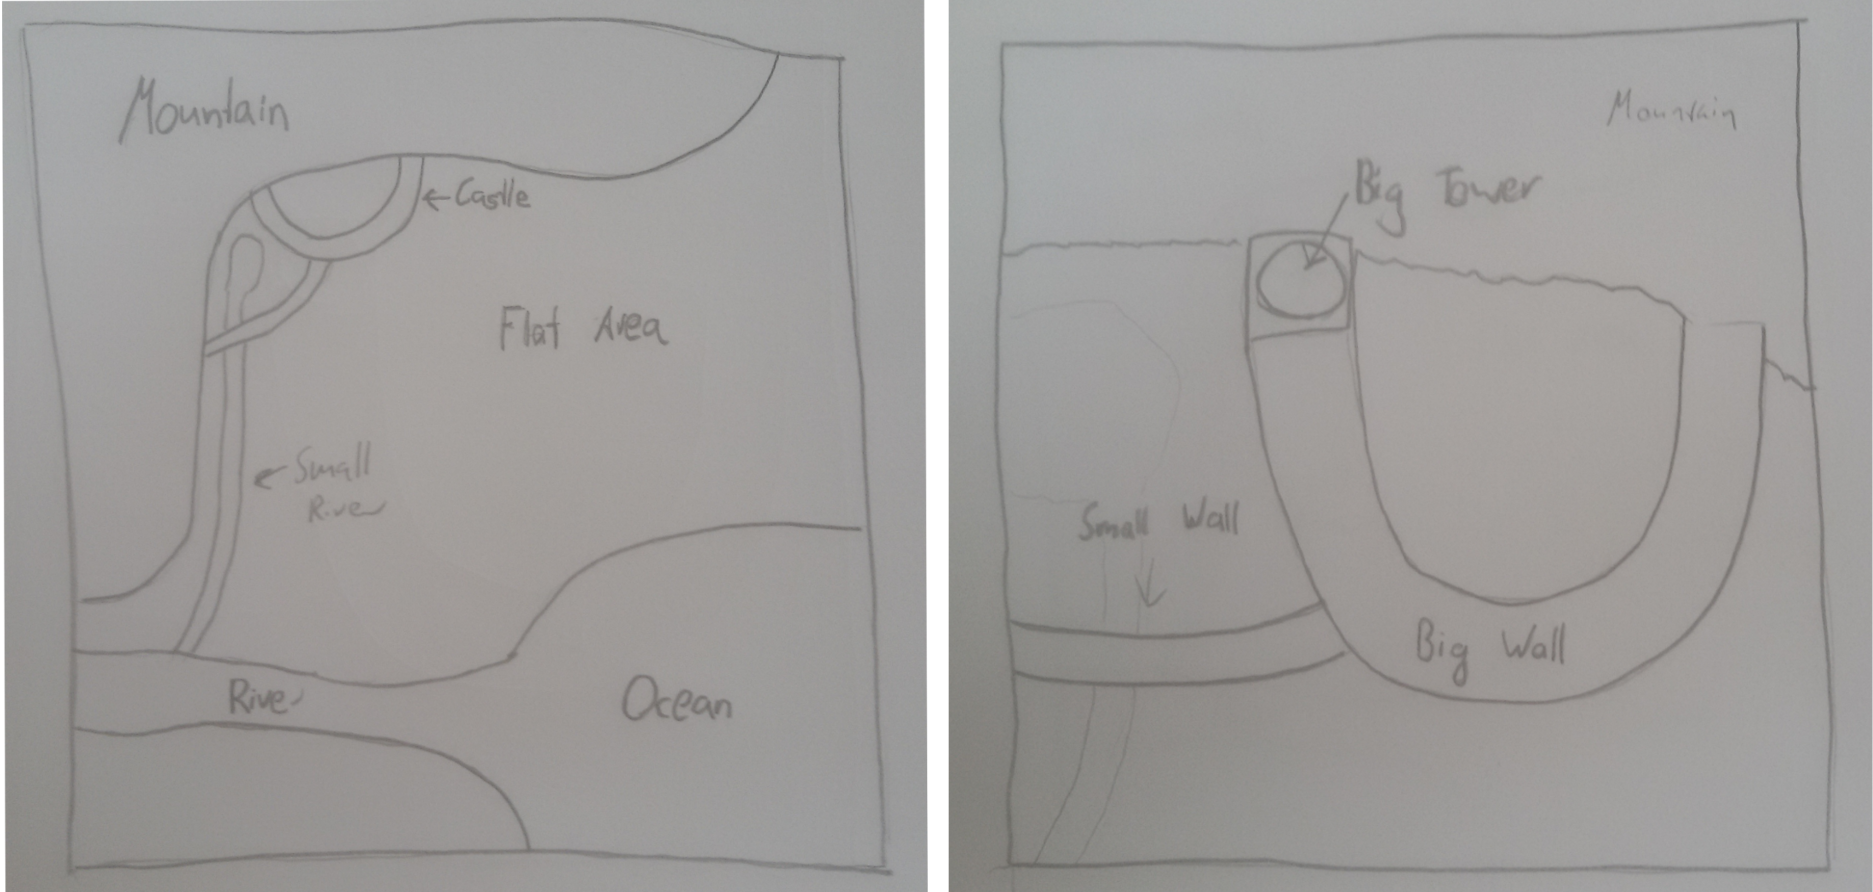
\includegraphics[width=0.95\linewidth]{Abbildungen/Unity/Skizzen}
	\caption{Handskizzen als Vorüberlegung}
	\label{handskizze}
\end{figure}


Die Größen wurden so festgelegt, dass sie begehbar ist und einen massiven Eindruck hinterlässt. Gesetze der realen Welt spielten beim Entwurf Burg keine Rolle. Auf Grundlage der gemeinsamen Überlegungen wurden die Abmessungen der Festung festgelegt und ein erstes Modell erstellt. Dieses war die Basis der gemeinsamen Projektarbeit und ermöglichte ein paralleles Arbeiten in Unity und 3d Studio Max.

Im Verlaufe der Arbeit wurden die beiden Teile immer wieder abgeglichen, Details hinzugefügt, das weitere Vorgehen besprochen und sukzessive entstand so die finale Szene. 